\documentclass{article}
\usepackage{iclr2027_conference}
\usepackage{times}
\usepackage{amsmath,amssymb,amsthm}
\usepackage{booktabs}
\usepackage{graphicx}
\usepackage{natbib}
\usepackage{hyperref}

\newtheorem{proposition}{Proposition}
\newtheorem{remark}{Remark}
\title{Beyond High Prices: Auditing Information-Mediated Enforcement in Recurrent Pricing Agents}
\author{Anonymous}

\begin{document}
\maketitle

\begin{abstract}
High prices do not by themselves show that pricing algorithms punish firms that undercut them. A price cut may lose money immediately, even when the rival never retaliates. We study this distinction in a continuous-price duopoly whose recurrent PPO agents receive noisy, delayed public reports instead of rival prices. Our audit freezes the trained policies, forces a one-period price cut, and separates its immediate profit effect from the discounted change in later profits. An action-independent report channel provides an exact zero-response negative control. Across ten training seeds per channel and one million training interactions per run, mean normalized price elevation ends at $0.015$ with informative reports and $0.019$ after channel replacement; the paired difference is $0.0037$ with a 95\% seed-bootstrap interval of $[-0.0241,0.0288]$. Almost all mean losses from the tested cuts arise immediately, and several small cuts remain profitable. A fixed-trigger model explains what a true continuation threat would require and why Gaussian noise weakens it under a fixed threshold. The evidence does not support learned punishment in these tested policies, while leaving other deviations, learners, and continuing markets open.
\end{abstract}

\section{Introduction}

Suppose two pricing algorithms charge more than the one-shot competitive price. One explanation is strategic: either firm could gain by cutting its price today, but it expects its rival to respond in a way that reduces future profits. Another explanation is simpler: the algorithms have not finished learning, or their current policies happen to choose high prices. Observing the price level cannot distinguish these explanations. Nor is every price cut a useful test of punishment. Near a firm's best-response price, a large cut can reduce profit on the same sale, before the rival has any chance to react.

We therefore ask a specific question: \emph{do trained pricing policies discourage unilateral price cuts through losses that occur later?} We call this mechanism information-mediated enforcement because a price cut must first change something the rival observes, and that information must then change future play. The relevant evidence is a chain from action to report, report to later actions, and later actions to continuation profit. High prices alone establish none of these links.

Our testbed is a duopoly with continuous prices and logit demand. Firms do not observe rival prices or profits while choosing actions. They receive a public report that averages two latent price signals, adds Gaussian noise, and arrives with a delay. Each firm uses proximal policy optimization (PPO) with a gated recurrent unit (GRU) to summarize a 32-report window. This is a controlled setting for studying finite-memory policies, rather than a claim about the architecture used by commercial pricing systems.

The audit has two parts. First, we freeze a trained policy pair and compare two otherwise matched rollouts: one follows the prescribed actions, and the other forces one firm to cut its price for a single period. We use the same monitoring draw and noise sequence in both branches. We then measure the current profit difference separately from all later discounted differences. Second, we retrain policies with public reports drawn independently of prices. Under the stated actor-input restrictions, this replacement gives an exact negative control: a forced action cannot affect later observations, actions, or profits.

The ten-seed results show near-Nash prices in both channels. The tested price cuts generally lose money immediately, while later losses are tiny. Some small cuts are profitable. There is a statistically resolved but economically small downward rival response under informative reports; a response of that size is not evidence that continuation losses offset a profitable current deviation. We also give a fixed public-trigger benchmark that states the incentive condition explicitly. Its role is to explain the mechanism the audit looks for, not to predict where neural training will converge.

\paragraph{Relation to earlier work.}
Repeated-game models explain how noisy public signals can support cooperation by changing future payoffs \citep{green1984noncooperative,abreu1990toward,fudenberg1994folk}. In algorithmic markets, \citet{calvano2020artificial} study tabular Q-learning with observable prices. \citet{calvano2021algorithmic} study quantity-setting Cournot learners with stochastic demand and public market-price signals, including forced output deviations. \citet{deng2025exploring} compare tabular Q-learning, DQN, and a discrete-action PPO variant in pricing markets. Our contribution is a payoff-decomposition audit for continuous-action, finite-memory PPO policies under delayed reports, together with a proved zero-response control. We do not claim that earlier studies lacked intervention tests or that our negative finding applies to all learners.

\section{Market, Reports, and Learning}

\subsection{A Stationary Pricing Market}

Two firms choose prices $p_{i,t}\in[1,2.5]$ simultaneously. Marginal cost is $c=1$, quality is $v=2$, market size is one, outside-option utility is zero, and the logit scale is $\mu=0.25$. Against rival $j$, demand and period profit are
\begin{align}
q_i(p_i,p_j)&=\frac{e^{(v-p_i)/\mu}}{1+e^{(v-p_i)/\mu}+e^{(v-p_j)/\mu}},\label{eq:demand}\\
\pi_i(p_i,p_j)&=(p_i-c)q_i(p_i,p_j).\label{eq:profit}
\end{align}
A lower price attracts more demand but reduces the margin on each unit. The one-shot Nash benchmark balances these effects for an individual firm. The joint-profit benchmark instead maximizes the firms' combined profit. The archived price-elevation measure uses grid references $p^{\mathrm N}=1.473$ and $p^{\mathrm J}=1.925$:
\begin{equation}
E=\frac{\bar p-p^{\mathrm N}}{p^{\mathrm J}-p^{\mathrm N}}.\label{eq:elevation}
\end{equation}
Thus $E=0$ is the Nash reference and $E=1$ is the joint-profit reference; values outside $[0,1]$ are allowed. Continuous first-order conditions give $1.4729266600$ and $1.9249809190$, respectively, but we retain the grid values actually used in the archived calculations (Supplement~B.1).

The archive also reports a field named \texttt{mean\_total\_surplus}. We call it the \emph{archived welfare index}: its values can be checked against saved outputs, but its simulator formula cannot be verified without the missing implementation. Standard logit total surplus and this reporting boundary are explained in Supplement~I.11. We do not infer a welfare improvement from this unverified field.

\subsection{What the Firms Observe}

At episode reset, a joint monitoring draw $\theta=(\theta_{\mathrm{lo}},\theta_{\mathrm{hi}},\sigma)$ is sampled from retained posterior rows and fixed for that episode. Prices determine a latent report mean:
\begin{equation}
m_t=\theta_{\mathrm{lo}}+(\theta_{\mathrm{hi}}-\theta_{\mathrm{lo}})
\operatorname{clip}\!\left(\frac{\min(p_{1,t},p_{2,t})-p^{\mathrm N}}{p^{\mathrm J}-p^{\mathrm N}},0,1\right).
\label{eq:latent}
\end{equation}
Taking the minimum makes the report sensitive to a unilateral cut. Clipping also creates a limitation: once either price is at or below $p^{\mathrm N}$, further cuts cannot lower $m_t$. A small observed response can therefore reflect signal saturation as well as a policy that ignores informative reports.

Under the informative channel, the generated report is
\begin{equation}
r_{t+1}=\tfrac12(m_t+m_{t-1})+\varepsilon_t,
\qquad\varepsilon_t\sim\mathcal N(0,\sigma_\varepsilon^2).
\label{eq:report}
\end{equation}
The effective innovation scale is denoted by $\sigma_\varepsilon$. Job files also record \texttt{added\_sigma}=0.1; the rule combining that setting with posterior $\sigma$ is unavailable and is not assumed here. The one-period report queue means that a price cut at $t$ can first affect an action at $t+2$. Delivered reports are centered at $1.6$, divided by $0.4$, and clipped to $[-5,5]$.

Under channel replacement, reports are instead drawn as $\mathcal N(1.6,0.4^2)$ independently of prices. The two firms still share the public draw, and delay and observation dimensions stay fixed. This intervention removes the price-to-report link, but it also changes the reports' marginal distribution and serial dependence. The retraining comparison therefore estimates the effect of the full replacement, rather than an information effect with all other input properties held fixed. Supplement~B gives the calibration description and the timing sequence.

\subsection{Learning and Deployment}

Each firm has its own actor--critic network and optimizer. A 128-unit GRU encodes the last 32 reports, starting from a fresh zero hidden state at each decision. The actor also receives normalized time $t/512$. It does not receive rival prices, current profits, or a separate own-action history. Reports can be ambiguous because of noise and delay; the GRU is a convenient way to process a short history, without asserting that it is necessary or superior to other encoders.

We use PPO \citep{schulman2017proximal} for $10^6$ joint market interactions per run in episodes of $T=512$ periods, with discount $\delta=0.99$ and no terminal-value bootstrap. Training samples actions from a $\tanh$-transformed Gaussian. Evaluation freezes the weights and uses $\tanh$ of the latent action mean. This deterministic rule need not equal the mean action of the stochastic training policy. All results below concern the frozen deterministic deployment. The full configuration, actor inputs, losses, and remaining implementation-verification limits appear in Supplement~C.

\section{An Audit That Separates Current and Later Effects}

\subsection{Paired One-Period Price Cuts}

For each policy pair, we intervene on either firm at $t_0\in\{64,256\}$. The forced action cuts are $0.1$ and $0.3$ on the normalized action scale, corresponding to unclipped price reductions of $0.075$ and $0.225$. Both firms return to their frozen policies after the intervention. This gives eight probe types per seed and 160 probes across ten seeds in each of two channels. Each probe averages 128 paired rollouts with the same posterior draw, initial report history, and noise innovations in the control and cut branches.

Let $d_t=\pi_t^{\mathrm{cut}}-\pi_t^{\mathrm{control}}$ be the deviator's period-profit difference. The full remaining-episode gain is
\begin{equation}
G=\underbrace{d_{t_0}}_{\text{immediate gain}}+
\underbrace{\sum_{t=t_0+1}^{T-1}\delta^{t-t_0}d_t}_{\Delta\pi^{\mathrm{cont}}:\ \text{continuation gain}}.
\label{eq:decomposition}
\end{equation}
A negative $G$ alone is not proof of punishment. If the immediate gain is already negative and the continuation term is zero, the cut loses money for a static reason. Evidence of deterrence would instead require a positive immediate gain offset by a sufficiently negative continuation term. Even then, that term contains both firms' later adjustments; it does not isolate retaliation by the rival on its own.

We also record the rival price difference $\Delta p_t^{\mathrm{rival}}=p_t^{\mathrm{rival,cut}}-p_t^{\mathrm{rival,control}}$. Its signed area sums the response after impact without discounting. A downward response describes a change in prices; Equation~\eqref{eq:decomposition} determines whether later profits actually deter the cut. Supplement~E defines these quantities and the uncertainty calculations precisely.

\subsection{Why the Replaced Channel Is a Negative Control}

\begin{proposition}[Observation invariance]\label{prop:invariance}
Suppose actors are frozen deterministic functions of public reports and time. Couple initial report buffers and innovations across branches. If reports are action independent, no other actor input depends on actions, and period payoffs depend only on current prices, then a one-period forced action leaves all later prescribed actions and payoffs unchanged. Hence $\Delta p_t^{\mathrm{rival}}=0$ for $t>t_0$ and $\Delta\pi^{\mathrm{cont}}=0$ pathwise.
\end{proposition}

\begin{proof}
The forced action does not change the next report or time input. Equal input histories give equal next actions. Repeating this argument gives equal future inputs and actions, and therefore equal future payoffs. Supplement~A.4 details the induction and its assumptions.
\end{proof}

This control checks a specific causal pathway. If own actions, rewards, sales, or a persistent economic state entered later inputs, an action could change the future even with action-independent public reports. Online weight updates would create another pathway. The proposition applies to the stated frozen-policy design, not arbitrary pricing agents. It also provides no positive-control test of how reliably the audit detects a genuinely collusive policy.

\section{What the Ten-Seed Results Show}

\subsection{Prices End Near the Static Benchmark}

We train ten seed pairs from scratch in each condition. Each run records 100 diagnostic evaluations of 16 episodes and a separate final evaluation of 64 episodes. Seeds, rather than episodes or checkpoints, are the unit of replication. Confidence intervals use 2,000 whole-seed bootstrap resamples; channel differences resample paired seed identifiers together. Supplement~D reports every seed and Supplement~E explains the intervals.

\begin{figure}[t]
\centering
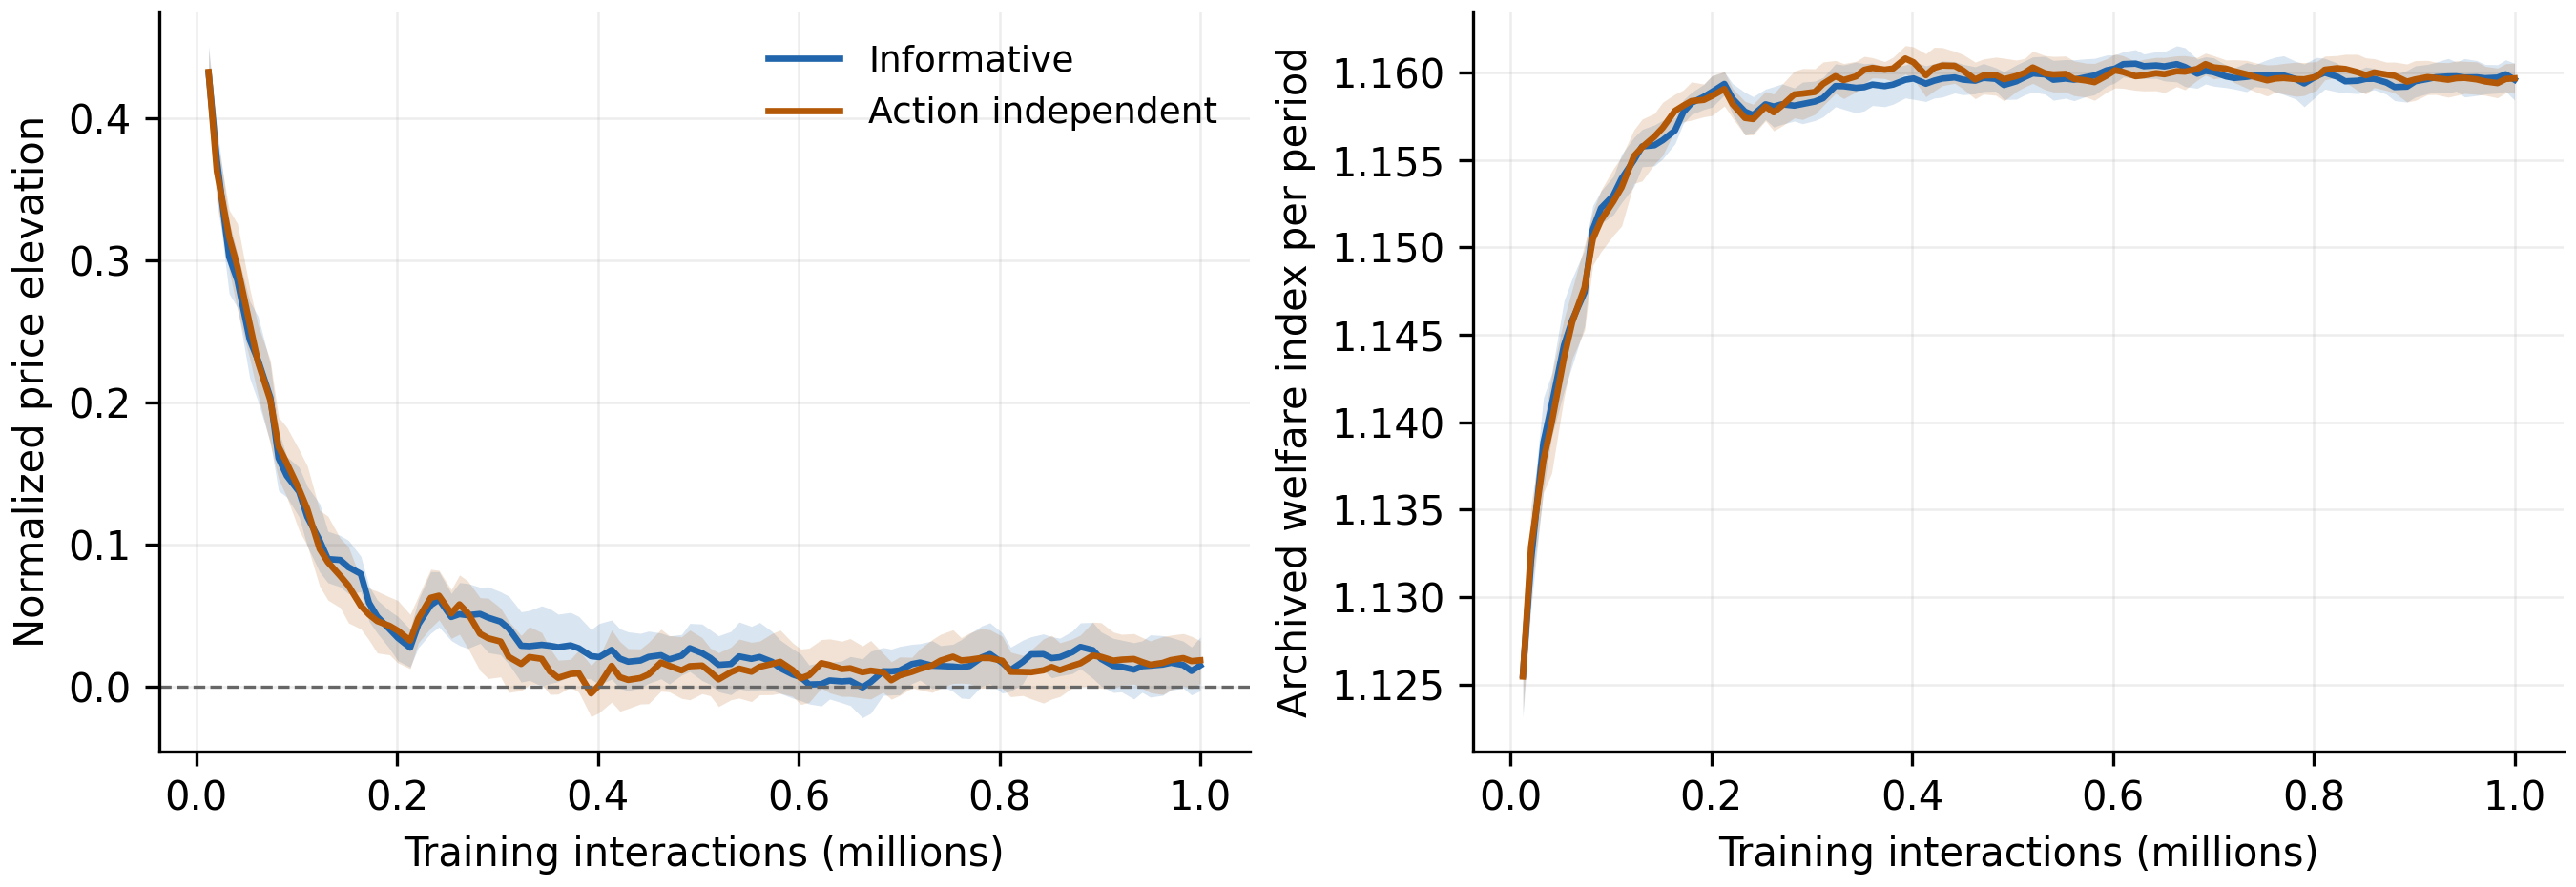
\includegraphics[width=\linewidth]{figures/image1.png}
\caption{Frozen deterministic deployment across training. Lines average ten seeds and bands are pointwise 95\% whole-seed bootstrap intervals. Left: normalized price elevation. Right: the archived welfare index, whose simulator definition remains unverified. These are diagnostic checkpoints, not new training replications.}
\label{fig:elevation}
\end{figure}

Mean elevation is about $0.43$ at the first recorded checkpoint, after $12{,}288$ training interactions, and declines overall with intermediate fluctuations (Figure~\ref{fig:elevation}). The first checkpoint is not an observation of the untrained initialization. At the final evaluation, mean elevation is $0.015052$ with informative reports and $0.018787$ with replaced reports (Table~\ref{tab:final}). The paired difference is small, but the interval includes effects of either sign. We do not claim equality, statistical equivalence, or an absence of every economically relevant effect.

\begin{table}[t]
\centering
\caption{Final evaluation over 64 episodes per seed, averaged across ten seeds. Differences are replaced minus informative. Intervals are paired-seed percentile bootstrap intervals, unadjusted across outcomes. The welfare field is reported as an archived index.}
\label{tab:final}
\small
\begin{tabular}{@{}lrrr@{}}
\toprule
Outcome & Informative & Replaced & Difference [95\% CI]\\
\midrule
Mean price & 1.479804 & 1.481492 & $0.001688\ [-0.0109,0.0130]$\\
Price elevation & 0.015052 & 0.018787 & $0.003735\ [-0.0241,0.0288]$\\
Archived welfare index & 1.159588 & 1.159660 & $0.000072\ [-0.0013,0.0017]$\\
Feature rank, firm 0 & 1.274335 & 1.338647 & $0.064312\ [0.0113,0.1337]$\\
Feature rank, firm 1 & 1.269538 & 1.353578 & $0.084040\ [0.0282,0.1495]$\\
\bottomrule
\end{tabular}
\end{table}

Feature rank is the exponential entropy of the normalized covariance eigenvalues of encoder features. Larger rank means activity is spread across more feature directions; it does not mean that a punishment rule has been learned. Rank is somewhat higher after replacement, but the input distribution and trained policies both change. This descriptive result identifies neither the cause of the rank difference nor a causal role for rank in pricing.

\subsection{Most Tested Losses Happen Immediately}

Table~\ref{tab:audit} separates immediate and full gains. Under informative reports, the mean full gain is $-0.005192$ for the smaller cut and $-0.051322$ for the larger cut. The continuation term is only about $-5\times10^{-6}$ in either case. Immediate losses account for $99.8983\%$ and $99.9897\%$ of the mean full loss, respectively. Large cuts near a best-response price can sacrifice margin immediately, so these negative full gains do not demonstrate a credible future threat.

\begin{figure}[t]
\centering
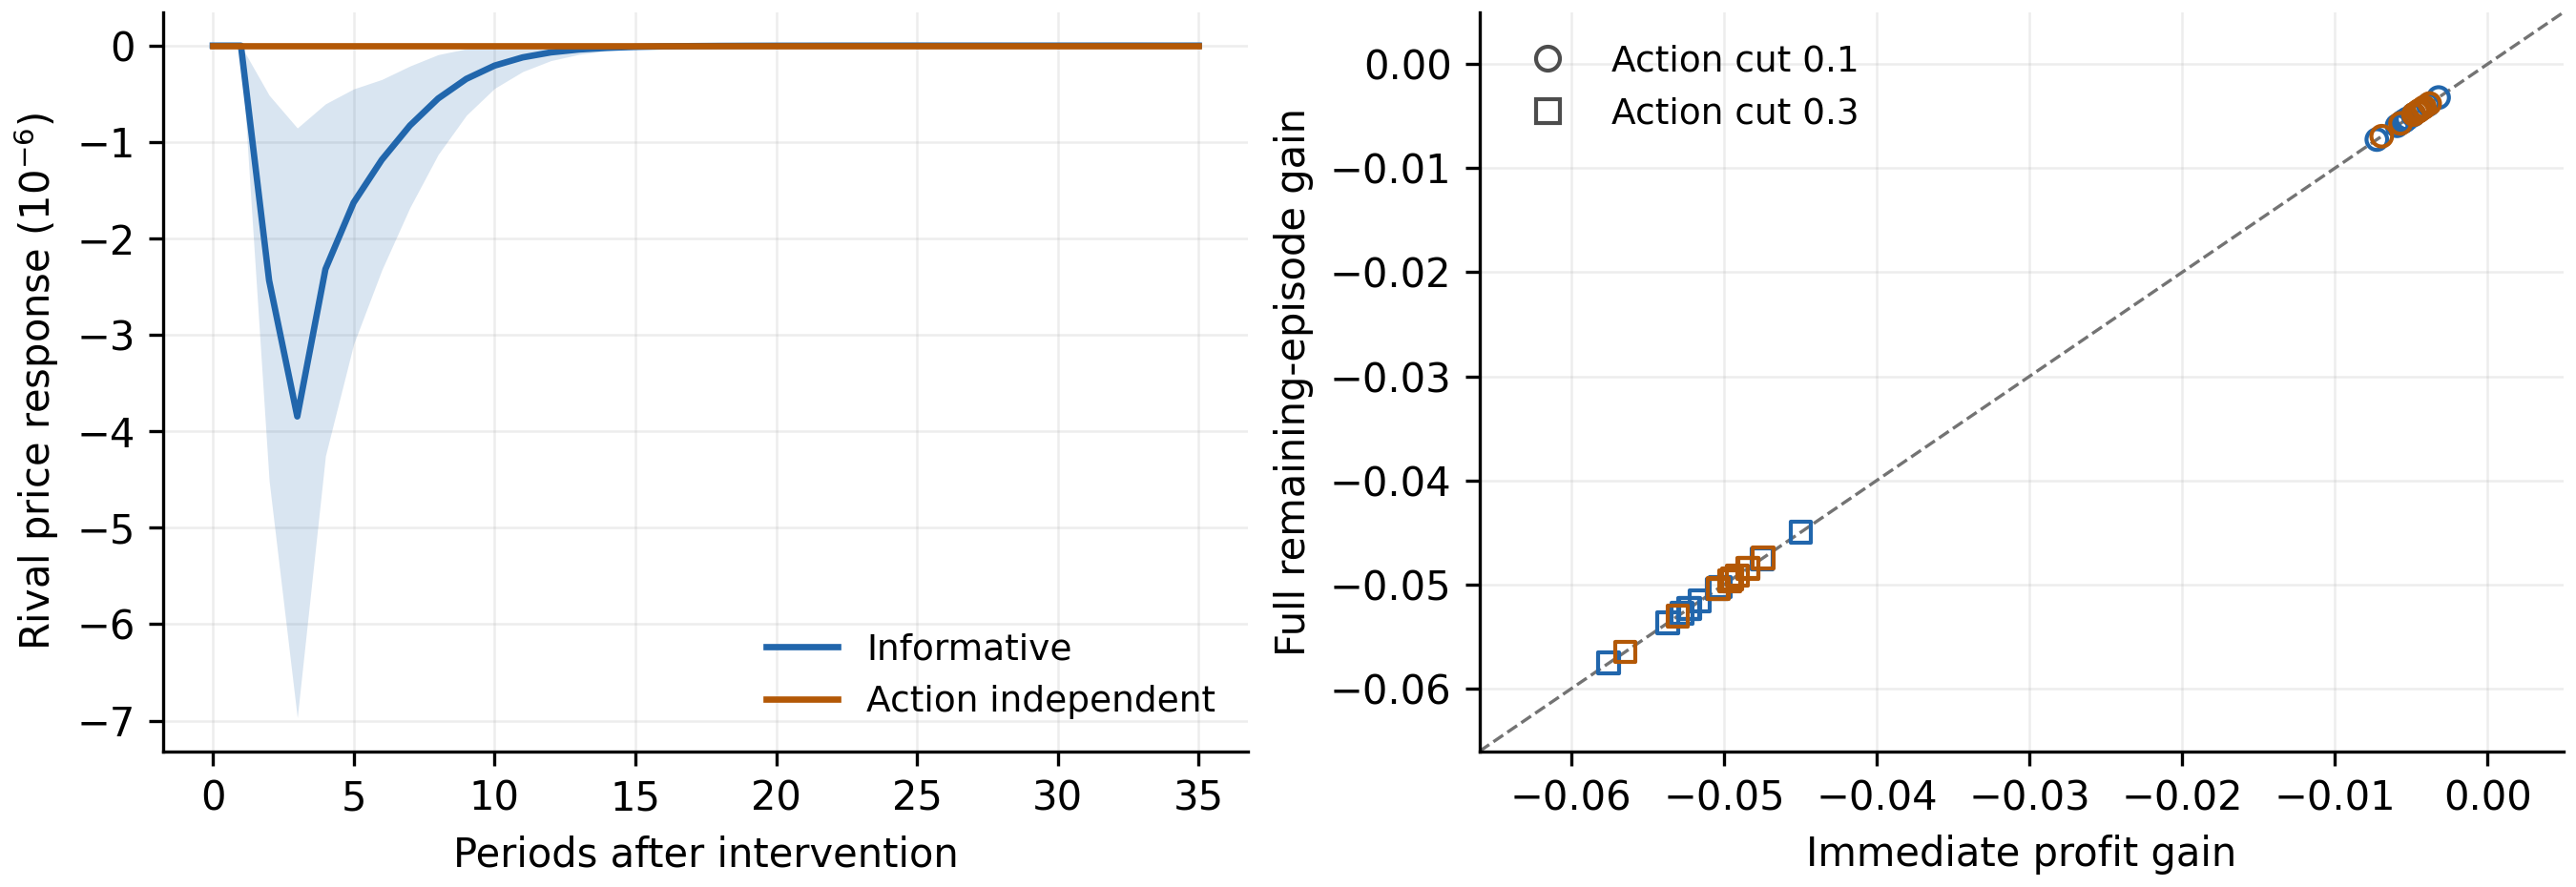
\includegraphics[width=\linewidth]{figures/image_2.png}
\caption{Price-cut audit. Left: mean rival response, averaging eight probe types within each seed before resampling seeds; bands are pointwise 95\% intervals. Only the first 36 lags are displayed. Right: immediate versus full gain, averaging four firm--time probes per cut and seed. Circles and squares denote cuts of $0.1$ and $0.3$. Continuation effects are too small to separate the points visibly from equality.}
\label{fig:deviation}
\end{figure}

\begin{table}[t]
\centering
\caption{Mean price-cut gains. Positive probes count positive conditional mean full gains among the 40 seed--firm--time probes per cut and channel; they are not multiplicity-adjusted discoveries.}
\label{tab:audit}
\begin{tabular}{@{}llrrr@{}}
\toprule
Channel & Cut & Immediate gain & Full gain & Positive probes\\
\midrule
Informative & 0.1 & $-0.005186$ & $-0.005192$ & 3 of 40\\
Informative & 0.3 & $-0.051317$ & $-0.051322$ & 0 of 40\\
Replaced & 0.1 & $-0.004800$ & $-0.004800$ & 1 of 40\\
Replaced & 0.3 & $-0.050273$ & $-0.050273$ & 0 of 40\\
\bottomrule
\end{tabular}
\end{table}

The informative rival response is small but not simply zero. Its mean signed area is $-1.36\times10^{-5}$ price-periods, with a 95\% seed-bootstrap interval of $[-2.53\times10^{-5},-3.42\times10^{-6}]$. This interval excludes zero. Nevertheless, a statistically detectable movement need not be large enough to discourage a profitable cut, and the payoff decomposition shows almost no continuation loss. Under replacement, all stored mean response paths are exactly zero and full and immediate gains agree to floating-point precision, consistent with Proposition~\ref{prop:invariance}.

The mean also hides useful exceptions. Three informative small-cut probes have positive mean gains, across two seeds, with a maximum of $0.003846$. One replaced-channel small-cut probe has mean gain $0.000122$. Their stored within-policy intervals exclude zero individually, without adjustment for testing many probes. These examples show why a negative average across cuts is not a certificate that every unilateral action is deterred. All 160 probe rows, including interval definitions, appear in Supplement~F; worked interpretations appear in Supplement~I.10.

\section{What a True Continuation Threat Would Require}

The audit's accounting has a simple repeated-game counterpart. Consider an infinite-horizon public strategy with a cooperative state $C$ and an absorbing punishment state $P$. The latter prescribes credible stage-game Nash play. Let the per-period payoff gap be $h=\pi^C-\pi^P>0$. A specified one-period deviation in $C$ gives a current gain $g=\pi^D-\pi^C>0$. A bad signal sends play to $P$: it occurs with probability $\alpha$ under cooperation and $\beta$ after the deviation. Assume $0\le\alpha<\beta\le1$ and $0\le\delta<1$.

Here $\alpha$ measures false alarms, while $\beta-\alpha$ measures how much more likely punishment becomes when the firm actually deviates. If the two probabilities are almost equal, the signal is a poor way to target a deviation. False alarms also make the cooperative future less valuable because punishment can arrive even when neither firm deviates.

\begin{proposition}[Specified-deviation threshold]\label{prop:threshold}
Under the fixed strategy above, the specified deviation is unprofitable exactly when
\begin{equation}
\delta\ge\delta^*=\frac{g}{g(1-\alpha)+(\beta-\alpha)h}.
\label{eq:threshold}
\end{equation}
Some admissible discount factor can deter it if and only if $(\beta-\alpha)h>\alpha g$. If $\beta\le\alpha$ and $g>0$, no discount factor below one can deter it.
\end{proposition}

The key value difference is $V^C-V^P=h/[1-\delta(1-\alpha)]$. The deviation's value is $g$ minus $\delta(\beta-\alpha)$ times that difference. Comparing these two terms gives Equation~\eqref{eq:threshold}; Supplement~A.1 supplies each Bellman step. Better detection and a larger payoff gap lower the required patience, while more false alarms raise it. The payoff gap $h$ is a difference between period profits, not the continuation-value difference $V^C-V^P$.

The proposition concerns one specified deviation. For firm $i$, let $g_i(a_i)$ be the current profit gain from action $a_i$, $h_i=\pi_i^C-\pi_i^P$ its cooperative payoff gap, and $\beta_i(a_i)$ the bad-signal probability after that action. Full incentive compatibility requires the comparison for \emph{every} firm and action:
\begin{equation}
g_i(a_i)[1-\delta(1-\alpha)]\le\delta[\beta_i(a_i)-\alpha]h_i.
\label{eq:full}
\end{equation}
A smaller current gain can be harder to deter if its detection probability is much lower. It is therefore not enough to check only the action giving the highest current profit. Supplement~A.2 gives an exact numerical example. Our two fixed cut sizes and two dates cannot establish Equation~\eqref{eq:full} over a continuous action space.

\subsection{Why Noise Weakens a Fixed Gaussian Trigger}

Suppose a contemporaneous signal has distribution $\mathcal N(\mu_C,\sigma^2)$ under cooperation and $\mathcal N(\mu_D,\sigma^2)$ after the specified deviation. Punishment follows when the signal is below a fixed threshold $\tau$, with $\mu_D<\tau<\mu_C$. Then
\[
\alpha=\Phi\bigl((\tau-\mu_C)/\sigma\bigr),\qquad
\beta=\Phi\bigl((\tau-\mu_D)/\sigma\bigr).
\]
\begin{proposition}[Restricted noise comparison]\label{prop:gauss}
Hold the means, threshold, actions, and payoff gaps fixed, with $\mu_D<\tau<\mu_C$. Increasing $\sigma>0$ raises false alarms, lowers detection, and strictly raises $\delta^*$ in Equation~\eqref{eq:threshold}.
\end{proposition}

More noise blurs the separation between the two signal distributions. A cooperative signal is more likely to cross the punishment threshold, while a deviating signal is more likely to escape it. Formally, $\alpha'(\sigma)>0$ and $\beta'(\sigma)<0$; combined with Proposition~\ref{prop:threshold}, these signs give the result. As noise tends to zero, the threshold tends to $g/(g+h)$. As noise tends to infinity, it tends to two, outside the feasible discount range. The full derivatives, limits, and the zero-added-noise boundary are in Supplement~A.3 and~I.9.

This benchmark makes an incentive mechanism explicit. It does not model the trained GRU as a binary trigger, and it does not show that PPO converges to that strategy. The experiment uses delayed, averaged reports and ends at a known date, whereas this benchmark uses a contemporaneous threshold and an infinite horizon. We compare their logic, not their equilibrium predictions.

\section{Interpretation and Limits}

The narrow finding is that these frozen PPO policies show no evidence that later losses enforce the tested price cuts. Early elevated prices decay toward the static benchmark, mean cut losses are overwhelmingly immediate, and several small cuts remain profitable. Neither the near-Nash mean nor the absence of a large continuation term establishes that every policy, history, or deviation is noncollusive.

Four design limits matter for interpreting this finding. First, replacing reports changes their distribution as well as their action dependence; a matched-distribution placebo would better isolate information content. Second, the latent-mean map saturates at the Nash boundary, which can hide the difference between two downward cuts. Third, the probe family omits upward, adaptive, and multistep deviations. Fourth, known $512$-period termination and time inputs make a different learning problem from an indefinitely continuing market. These are substantive restrictions, not reasons to treat an unresolved effect as exactly zero.

There is also a measurement limit: a zero-response negative control validates invariance under the stated design, but cannot establish sensitivity to a genuinely collusive policy. A known positive-control trigger with a profitable immediate deviation and a larger continuation loss would test that sensitivity. Such controls, additional learners, and alternative monitoring maps remain future experiments; none is presented as completed here. Supplement~H discusses each limit and Supplement~I connects it to the main argument.

\paragraph{Conclusion.}
To assess dynamic enforcement, ask what the firm gains now and what it loses later. Our paired price-cut audit makes that distinction explicit and checks a pathway through public information. In this testbed, the observed losses come almost entirely from the price cut itself, rather than a future threat. The broader lesson is methodological: a price level, an impulse-response plot, and an incentive-compatible punishment mechanism are different kinds of evidence.

\section*{Reproducibility Statement}
Supplement~A provides derivations; B--C describe monitoring and training; D--F report seed outcomes, uncertainty conventions, and every probe; G documents artifact identities and computation; I gives a detailed walkthrough. The archived tables and checkpoint hashes can be rechecked with the supplied postprocessing scripts. Original training/simulator code, calibration inputs, posterior draws, and individual-rollout data are unavailable, so full training and MCMC replication remains unverified. No new policies were trained for this revision.

\clearpage
\bibliographystyle{iclr2027_conference}
\begin{thebibliography}{9}

\bibitem[Abreu et~al.(1990)]{abreu1990toward}
D.~Abreu, D.~Pearce, and E.~Stacchetti.
\newblock Toward a theory of discounted repeated games with imperfect
  monitoring.
\newblock \emph{Econometrica}, 58(5):1041--1063, 1990.

\bibitem[Calvano et~al.(2020)]{calvano2020artificial}
E.~Calvano, G.~Calzolari, V.~Denicol\`o, and S.~Pastorello.
\newblock Artificial intelligence, algorithmic pricing, and collusion.
\newblock \emph{American Economic Review}, 110(10):3267--3297, 2020.

\bibitem[Calvano et~al.(2021)]{calvano2021algorithmic}
E.~Calvano, G.~Calzolari, V.~Denicol\`o, and S.~Pastorello.
\newblock Algorithmic collusion with imperfect monitoring.
\newblock \emph{International Journal of Industrial Organization}, 79:102712,
  2021.

\bibitem[Deng et~al.(2025)]{deng2025exploring}
S.~Deng, M.~Schiffer, and M.~Bichler.
\newblock Exploring competitive and collusive behaviors in algorithmic
  pricing with deep reinforcement learning.
\newblock \emph{arXiv preprint arXiv:2503.11270}, 2025.

\bibitem[Fudenberg et~al.(1994)]{fudenberg1994folk}
D.~Fudenberg, D.~K.~Levine, and E.~Maskin.
\newblock The folk theorem with imperfect public information.
\newblock \emph{Econometrica}, 62(5):997--1039, 1994.

\bibitem[Green and Porter(1984)]{green1984noncooperative}
E.~J.~Green and R.~H.~Porter.
\newblock Noncooperative collusion under imperfect price information.
\newblock \emph{Econometrica}, 52(1):87--100, 1984.

\bibitem[Schulman et~al.(2017)]{schulman2017proximal}
J.~Schulman, F.~Wolski, P.~Dhariwal, A.~Radford, and O.~Klimov.
\newblock Proximal policy optimization algorithms.
\newblock \emph{arXiv preprint arXiv:1707.06347}, 2017.

\bibitem[Vehtari et~al.(2021)]{vehtari2021rank}
A.~Vehtari, A.~Gelman, D.~Simpson, B.~Carpenter, and P.-C.~B\"urkner.
\newblock Rank-normalization, folding, and localization: An improved
  $\hat{R}$ for assessing convergence of {MCMC}.
\newblock \emph{Bayesian Analysis}, 16(2):667--718, 2021.

\end{thebibliography}

\section*{AI Use Statement}
Generative AI assisted with writing, explanation, mathematical checks, and postprocessing of archived outputs. It did not supply hypothetical experimental results. The authors are responsible for all assumptions, derivations, references, reported results, and limitations.

\end{document}
